% Section 7: Performance Evaluation Metrics (Slides 48-60)

% Slide 48: Model Evaluation
\begin{frame}{ارزیابی مدل‌های طبقه‌بندی}{\lr{Model Evaluation}}
  \begin{columns}[T]
    \begin{column}{0.54\textwidth}
      \begin{itemize}
        \setlength{\itemsep}{8pt}
        \item \textbf{پرسش بنیادین:} مدل ساخته‌شده در طبقه‌بندی رکوردهای جدید و نادیده چقدر موفق است؟ (\lr{Generalization Performance})
        \item \textbf{موضوع این بخش: معیارهای ارزیابی}
        \begin{itemize}
          \setlength{\itemsep}{4pt}
          \item عملکرد مدل را چگونه به شکل کمّی اندازه بگیریم؟
          \item کدام معیار برای مسائل نامتوازن یا حساس به هزینه مناسب است؟
        \end{itemize}
      \end{itemize}
    \end{column}
    \begin{column}{0.44\textwidth}
      \begin{center}
        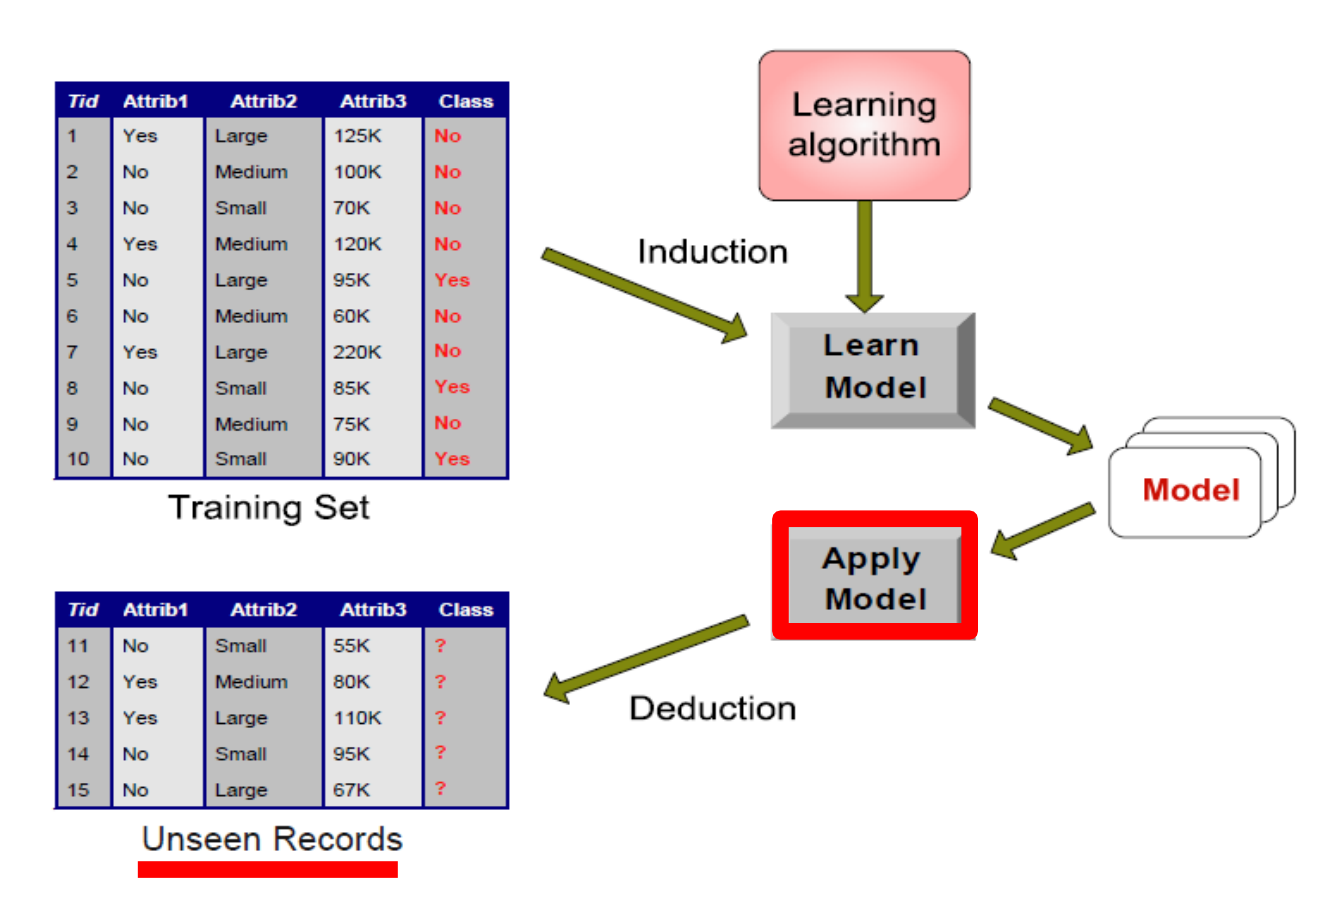
\includegraphics[width=\textwidth,height=4.8cm,keepaspectratio]{images/slide48_evaluation_overview.png}
      \end{center}
    \end{column}
  \end{columns}
\end{frame}

% Slide 49: Confusion Matrix
\begin{frame}{ماتریس درهم‌ریختگی}{\lr{Confusion Matrix}}
  \begin{itemize}
    \setlength{\itemsep}{3pt}
    \item تمرکز بر توان پیش‌بینی مدل با بررسی نمونه‌های درست و نادرست:
    \begin{itemize}
      \item مسئله دوکلاسه (کلاس مثبت / منفی)
      \item \textbf{واژه اول:} \lr{(True / False)} درستی پیش‌بینی (اگر پیش‌بینی درست باشد \lr{True}، در غیر این صورت \lr{False})
      \item \textbf{واژه دوم:} \lr{(Positive / Negative)} وابسته به برچسب پیش‌بینی‌شده توسط مدل
    \end{itemize}
  \end{itemize}
  \vspace{0.2cm}
  \begin{center}
    \renewcommand{\arraystretch}{1.25}
    \small
    \begin{tabular}{|c|c|c|c|}
      \hline
      \multicolumn{2}{|c|}{} & \multicolumn{2}{c|}{\textbf{کلاس پیش‌بینی‌شده (\lr{Predicted})}} \\
      \cline{3-4}
      \multicolumn{2}{|c|}{} & \textbf{\lr{Class = Yes}} & \textbf{\lr{Class = No}} \\
      \hline
      \multirow{2}{*}{\textbf{\lr{Actual}}} & \textbf{\lr{Class = Yes}} & 
      \begin{tabular}{c}\textbf{مثبت واقعی (\lr{TP})}\\\footnotesize \lr{True Positives}\end{tabular} & 
      \begin{tabular}{c}\textbf{منفی کاذب (\lr{FN})}\\\footnotesize \lr{False Negatives}\end{tabular} \\
      \cline{2-4}
      & \textbf{\lr{Class = No}} & 
      \begin{tabular}{c}\textbf{مثبت کاذب (\lr{FP})}\\\footnotesize \lr{False Positives}\end{tabular} & 
      \begin{tabular}{c}\textbf{منفی واقعی (\lr{TN})}\\\footnotesize \lr{True Negatives}\end{tabular} \\
      \hline
    \end{tabular}
  \end{center}
\end{frame}

% Slide 50: Metrics for Performance Evaluation
\begin{frame}{معیارهای پایه ارزیابی عملکرد}{\lr{Metrics for Performance Evaluation}}
  \begin{columns}[T]
    \begin{column}{0.48\textwidth}
      \begin{block}{صحت کلی \ \lr{(Accuracy)}}
        \[
          \text{Accuracy} = \frac{TP + TN}{TP + TN + FP + FN}
        \]
        نسبت تمام پیش‌بینی‌های درست به کل نمونه‌ها
      \end{block}
      \begin{block}{نرخ خطا \ \lr{(Error Rate)}}
        \[
          \text{Error Rate} = 1 - \text{Accuracy}
        \]
      \end{block}
    \end{column}
    \begin{column}{0.48\textwidth}
      \begin{block}{نرخ مثبت واقعی \ \lr{(TPR / Recall)}}
        \[
          \text{TPR} = \frac{TP}{TP + FN}
        \]
        کسری از مثبت‌های واقعی که به درستی کشف شدند
      \end{block}
      \begin{block}{نرخ مثبت کاذب \ \lr{(FPR)}}
        \[
          \text{FPR} = \frac{FP}{FP + TN}
        \]
        کسری از منفی‌ها که به اشتباه مثبت پیش‌بینی شدند
      \end{block}
    \end{column}
  \end{columns}
\end{frame}

% Slide 51: What is a Good Accuracy?
\begin{frame}{صحت مطلوب چقدر است؟}{\lr{What is a Good Accuracy?}}
  \begin{itemize}
    \setlength{\itemsep}{6pt}
    \item یعنی چه زمانی کار آموزش به پایان رسیده است؟
    \begin{itemize}
      \item در صحت \lr{75\%}؟ \lr{90\%}؟ \lr{95\%}؟
    \end{itemize}
    \vspace{0.15cm}
    \item بستگی به درجه سختی مسئله دارد!
    \item \textbf{خط مبنا (\lr{Baseline})} -- حدس ساده‌لوحانه (\lr{Naive Guessing})
    \begin{itemize}
      \item همواره کلاس اکثریت را پیش‌بینی کنیم
    \end{itemize}
    \vspace{0.15cm}
    \item \textbf{مقایسه کنید:}
    \begin{itemize}
      \item پیش‌بینی پرتاب سکه با صحت \lr{50\%}
      \item پیش‌بینی پرتاب تاس با صحت \lr{50\%}
      \item پیش‌بینی اعداد قرعه‌کشی لوتو (۶ از ۴۹) با صحت \lr{50\%}
    \end{itemize}
  \end{itemize}
\end{frame}

% Slide 52: Limitation of Accuracy: Unbalanced Data
\begin{frame}{محدودیت صحت در داده‌های نامتوازن}{\lr{Limitation of Accuracy: Unbalanced Data}}
  \begin{itemize}
    \setlength{\itemsep}{5pt}
    \item کلاس‌ها اغلب فراوانی بسیار نابرابری دارند:
    \begin{itemize}
      \item تشخیص تقلب: \lr{98\%} تراکنش‌ها عادی، \lr{2\%} تقلب
      \item تجارت الکترونیک: \lr{99\%} بازدیدکنندگان خرید نمی‌کنند، \lr{1\%} خرید می‌کنند
    \end{itemize}
    \vspace{0.15cm}
    \item یک مسئله دوکلاسه را در نظر بگیرید:
    \begin{itemize}
      \item تعداد نمونه‌های منفی = \lr{9,990}، تعداد نمونه‌های مثبت = \lr{10}
      \item اگر مدل تمام نمونه‌ها را متعلق به کلاس منفی پیش‌بینی کند:
      \[
        \text{Accuracy} = \frac{9990}{10000} = 99.9\%
      \]
      \item صحت کاملاً گمراه‌کننده است زیرا مدل \textbf{حتی یک نمونه مثبت را هم کشف نکرده است!}
    \end{itemize}
  \end{itemize}
\end{frame}

% Slide 53: Precision and Recall
\begin{frame}{دقت و بازخوانی}{\lr{Precision and Recall}}
  \begin{columns}[c]
    \begin{column}{0.60\textwidth}
      \begin{itemize}
        \setlength{\itemsep}{5pt}
        \item \textbf{دقت (\lr{Precision}):}
        \[
          p = \frac{TP}{TP + FP}
        \]
        از میان مواردی که مثبت طبقه‌بندی شدند، چه کسری واقعاً مثبت هستند؟
        \vspace{0.1cm}
        \item \textbf{بازخوانی (\lr{Recall}):}
        \[
          r = \frac{TP}{TP + FN}
        \]
        کدام کسر از کل نمونه‌های مثبت، به درستی طبقه‌بندی شده‌اند؟
      \end{itemize}
    \end{column}
    \begin{column}{0.38\textwidth}
      \centering
      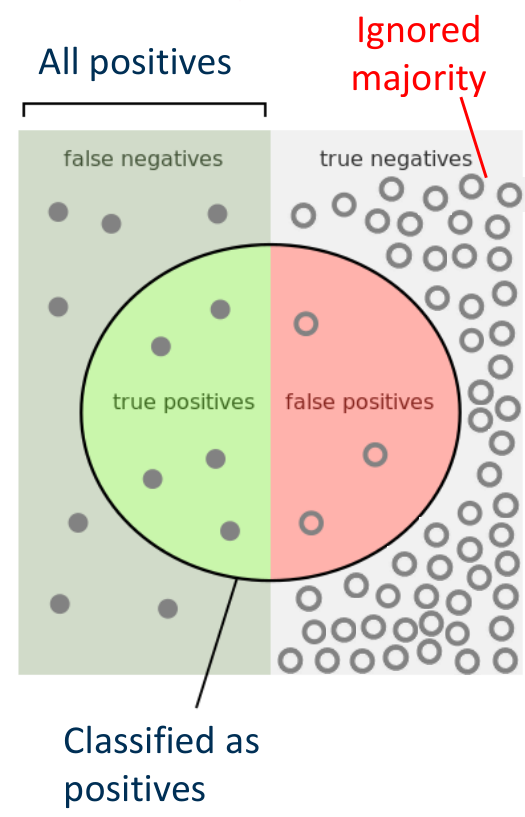
\includegraphics[width=\textwidth,height=5.5cm,keepaspectratio]{images/slide53_walber_full_clean.png}
    \end{column}
  \end{columns}
\end{frame}

% Slide 54: Precision and Recall - A Problematic Case
\begin{frame}{دقت و بازخوانی: یک نمونه مسئله‌ساز}{\lr{Precision and Recall -- A Problematic Case}}
  \begin{columns}[T]
    \begin{column}{0.48\textwidth}
      \begin{block}{ماتریس درهم‌ریختگی نمونه}
        \centering\footnotesize
        \begin{tabular}{|c|c|c|}
          \hline
          & \textbf{واقعی +} & \textbf{واقعی -} \\
          \hline
          \textbf{پیش‌بینی +} & $TP = 1$ & $FP = 0$ \\
          \hline
          \textbf{پیش‌بینی -} & $FN = 99$ & $TN = 1000$ \\
          \hline
        \end{tabular}
      \end{block}
      \vspace{0.2cm}
      \begin{itemize}
        \setlength{\itemsep}{5pt}
        \item $\text{Precision} = \frac{1}{1 + 0} = \mathbf{100\%}$
        \item $\text{Recall} = \frac{1}{1 + 99} = \mathbf{1\%}$
      \end{itemize}
    \end{column}
    \begin{column}{0.48\textwidth}
      \begin{alertblock}{تحلیل نتیجه}
        \begin{itemize}
          \setlength{\itemsep}{4pt}
          \item مدل دقت \lr{100\%} دارد زیرا هیچ نمونه منفی را اشتباهاً مثبت پیش‌بینی نکرده است!
          \item اما ۹۹ مورد مثبت از ۱۰۰ مورد را کاملاً از دست داده است (\lr{Recall = 1\%})!
          \item \textbf{نتیجه:} نیازمند معیاری هستیم که دقت و بازخوانی را با هم ترکیب کند و فقط در صورت بالا بودن هر دو، مقدار بزرگی داشته باشد.
        \end{itemize}
      \end{alertblock}
    \end{column}
  \end{columns}
\end{frame}

% Slide 55: F1-Measure
\begin{frame}{معیار $F_1$}{\lr{F1-Measure}}
  \begin{itemize}
    \item \textbf{تعریف:} معیار $F_1$ میانگین همساز (\lr{Harmonic Mean}) دقت و بازخوانی است:
    \[
      F_1 = 2 \cdot \frac{\text{Precision} \cdot \text{Recall}}{\text{Precision} + \text{Recall}}
    \]
    \item \textbf{خاصیت میانگین همساز:} همواره به مقدار کوچکتر گرایش دارد؛ بنابراین برای بالا بودن $F_1$، باید \textbf{هم دقت و هم بازخوانی هم‌زمان بالا باشند}.
  \end{itemize}
  \vspace{0.05cm}
  \begin{columns}[T]
    \begin{column}{0.48\textwidth}
      \begin{center}
        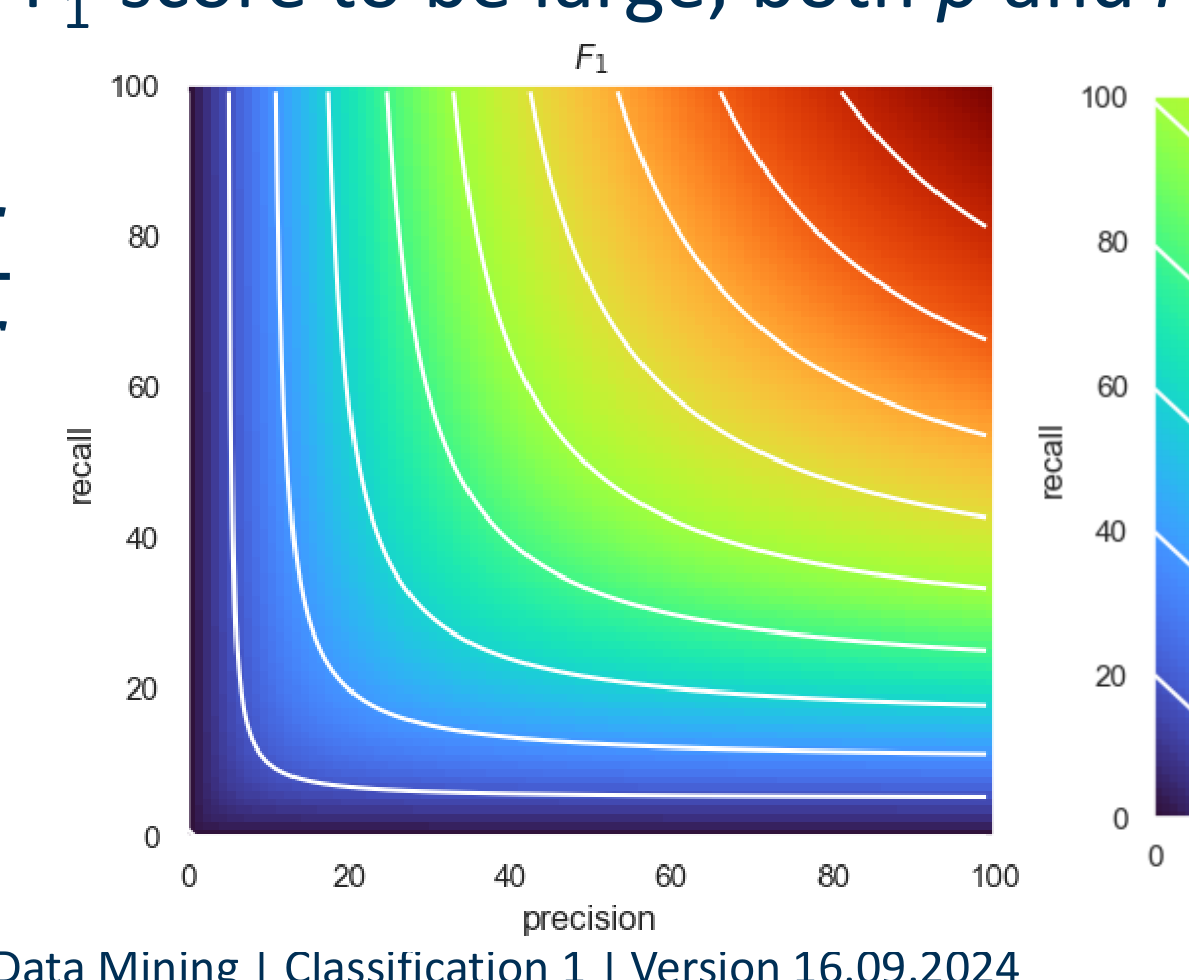
\includegraphics[width=\textwidth,height=3.4cm,keepaspectratio]{images/slide55_f1_3d.png}
      \end{center}
    \end{column}
    \begin{column}{0.48\textwidth}
      \begin{center}
        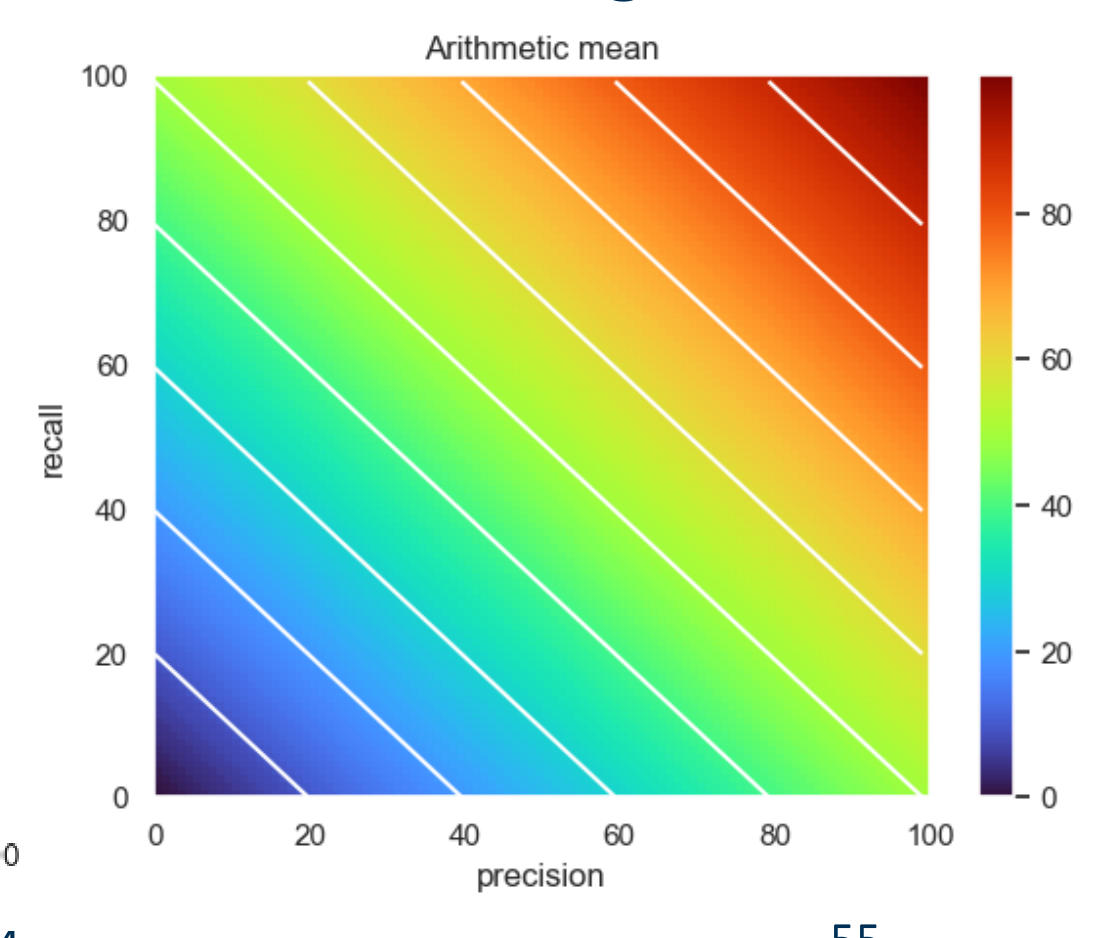
\includegraphics[width=\textwidth,height=3.4cm,keepaspectratio]{images/slide55_f1_contour.png}
      \end{center}
    \end{column}
  \end{columns}
\end{frame}

% Slide 56: F1-Measure Graph
\begin{frame}{نمودار معیار $F_1$ و آستانه بهینه}{\lr{F1-Measure Graph}}
  \begin{itemize}
    \item با تغییر آستانه تصمیم‌گیری:
    \begin{itemize}
      \item آستانه پایین: بازخوانی بالا ولی دقت پایین
      \item آستانه سخت‌گیرانه: دقت بالا ولی بازخوانی پایین
    \end{itemize}
    \item نقطه بهینه با بیشینه‌سازی نمره $F_1$ تعیین می‌شود:
  \end{itemize}
  \vspace{0.1cm}
  \begin{center}
    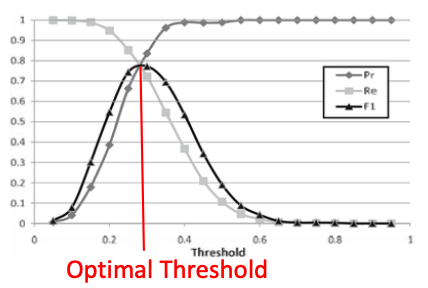
\includegraphics[width=0.72\textwidth,height=3.8cm,keepaspectratio]{images/slide56_f1_graph_clean.png}
  \end{center}
\end{frame}

% Slide 57: F_beta-Measure
\begin{frame}{معیار تعمیم‌یافته $F_\beta$}{\lr{F-beta Measure}}
  \begin{itemize}
    \setlength{\itemsep}{3pt}
    \item وزن‌دهی انعطاف‌پذیر به دقت در برابر بازخوانی:
    \[
      F_\beta = (1 + \beta^2) \cdot \frac{\text{Precision} \cdot \text{Recall}}{(\beta^2 \cdot \text{Precision}) + \text{Recall}}
    \]
    \item اگر $\beta = 2$: بازخوانی اهمیت بالاتری دارد (تشخیص بیماری یا کلاهبرداری).
    \item اگر $\beta = 0.5$: دقت اهمیت بالاتری دارد (سامانه‌های پیشنهادگر یا فیلتر هرزنامه).
  \end{itemize}
  \vspace{0.05cm}
  \begin{columns}[T]
    \begin{column}{0.48\textwidth}
      \begin{center}
        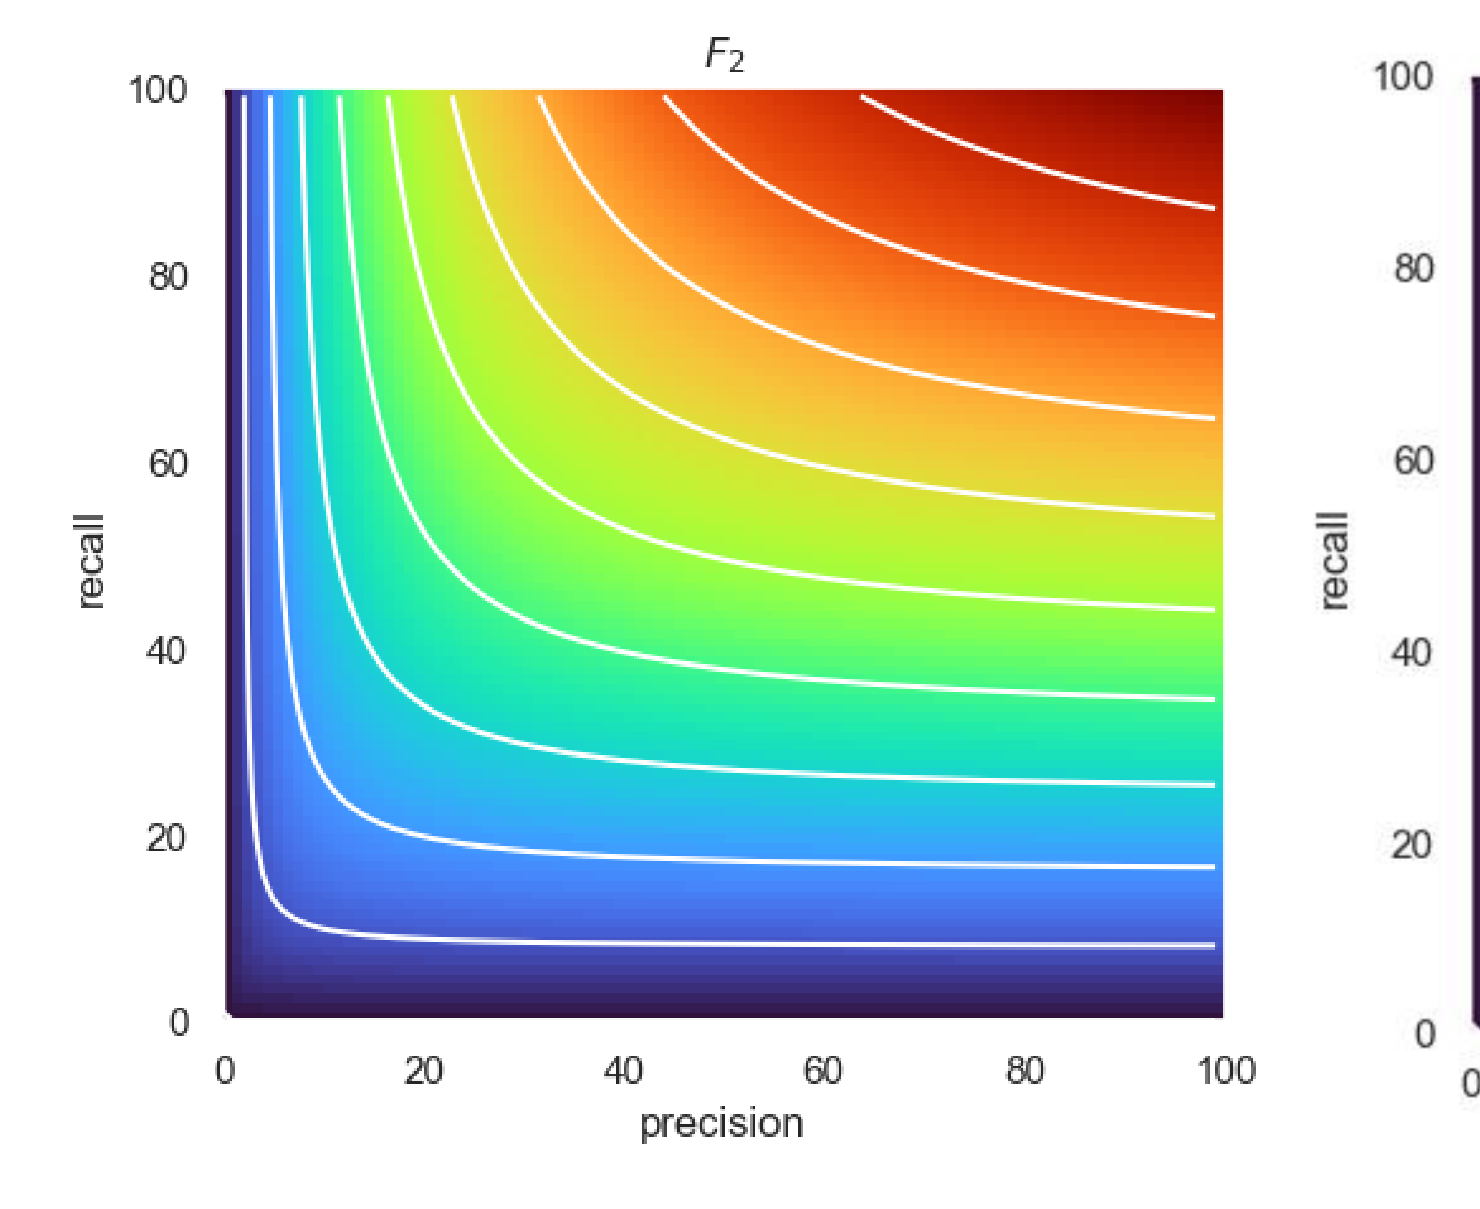
\includegraphics[width=\textwidth,height=2.5cm,keepaspectratio]{images/slide57_fbeta_curves.png}
      \end{center}
    \end{column}
    \begin{column}{0.48\textwidth}
      \begin{center}
        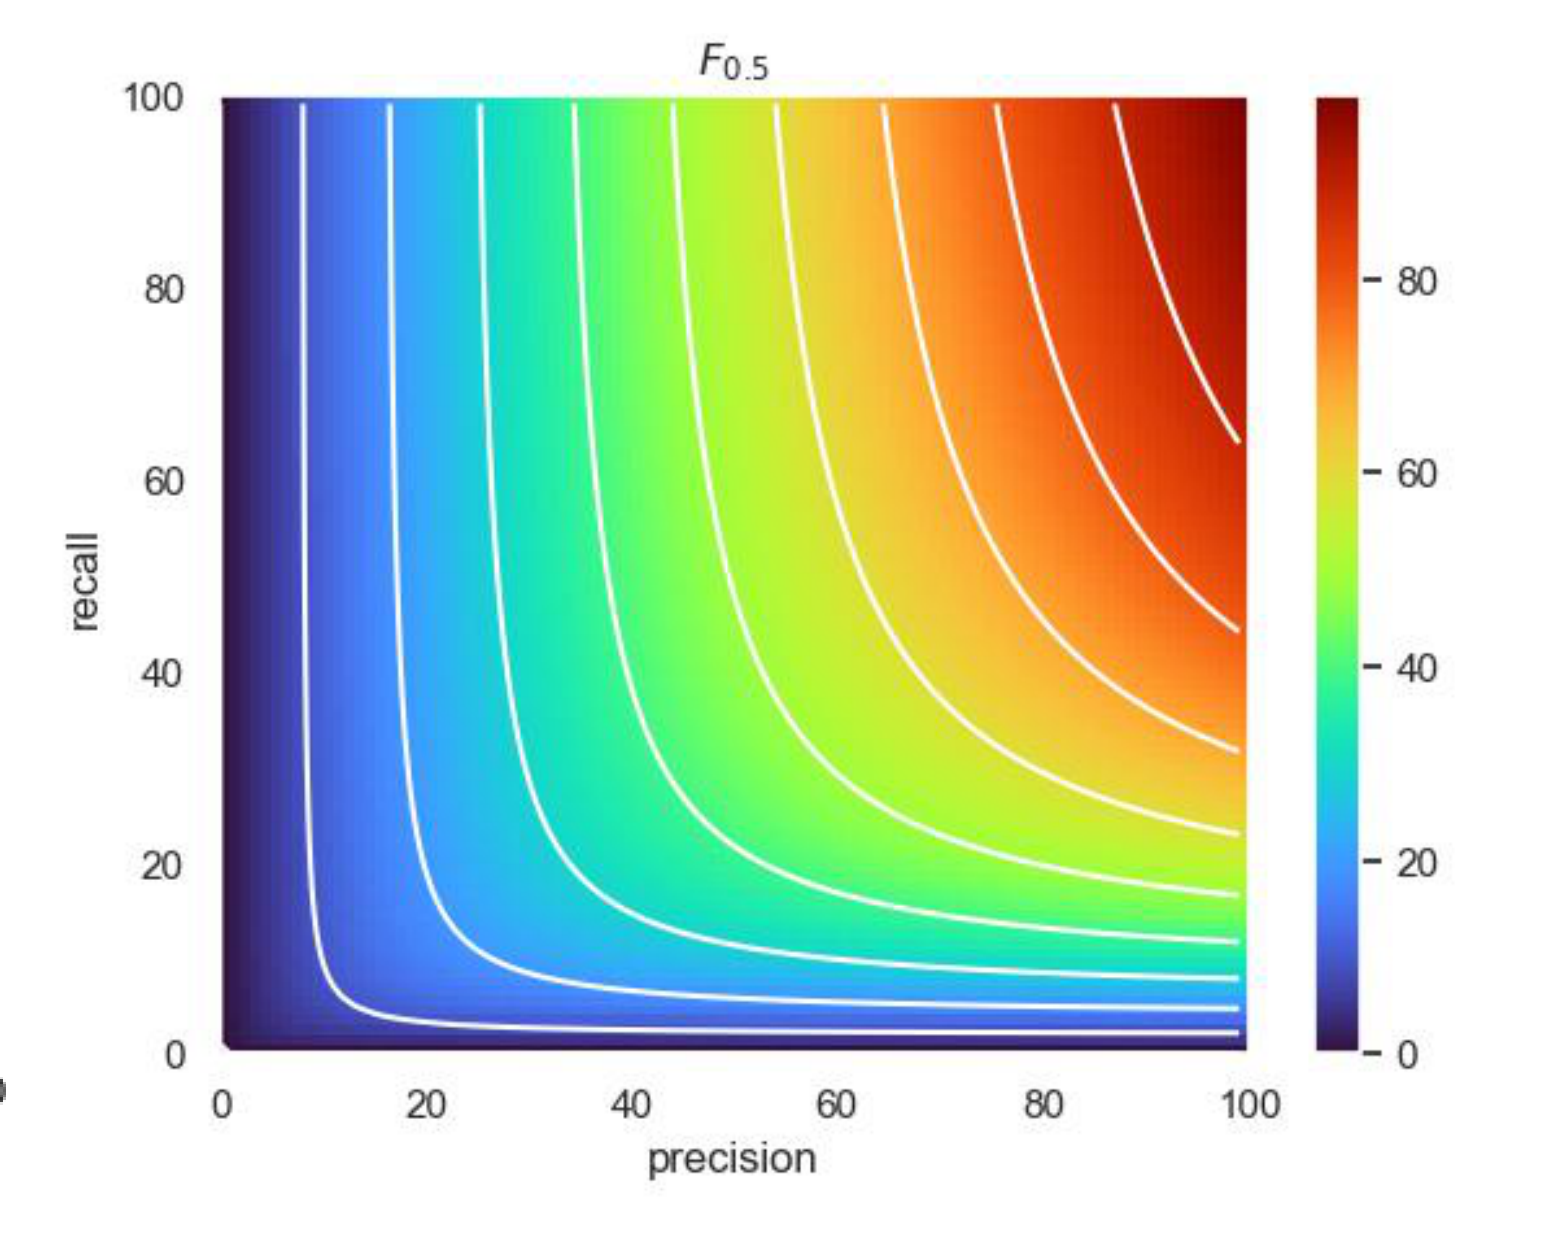
\includegraphics[width=\textwidth,height=2.5cm,keepaspectratio]{images/slide57_fbeta_surfaces.png}
      \end{center}
    \end{column}
  \end{columns}
\end{frame}

% Slide 58: Cost-Sensitive Model Evaluation
\begin{frame}{ارزیابی مدل مبتنی بر ماتریس هزینه}{\lr{Cost-Sensitive Model Evaluation}}
  \begin{columns}[T]
    \begin{column}{0.54\textwidth}
      \begin{itemize}
        \setlength{\itemsep}{4pt}
        \item تخصیص هزینه برای هر خطا (\lr{Cost for each error})
        \item \textbf{مورد کاربرد:} تشخیص تقلب در کارت‌های اعتباری
        \begin{itemize}
          \item ندیدن تراکنش‌های متقلبانه بسیار پرهزینه است ($FN$).
          \item هشدارهای اشتباه هزینه اندکی دارند ($FP$).
        \end{itemize}
      \end{itemize}
    \end{column}
    \begin{column}{0.44\textwidth}
      \centering\scriptsize
      \textbf{ماتریس هزینه (\lr{Cost Matrix})}\\[2pt]
      \begin{tabular}{|c|c|c|}
        \hline
        & \multicolumn{2}{c|}{\textbf{\lr{Predicted}}} \\
        \cline{2-3}
        \textbf{\lr{Actual}} & \textbf{\lr{Yes}} & \textbf{\lr{No}} \\
        \hline
        \textbf{\lr{Yes}} & -1 & 100 \\
        \hline
        \textbf{\lr{No}} & 1 & 0 \\
        \hline
      \end{tabular}
    \end{column}
  \end{columns}
  \vspace{0.25cm}
  \begin{columns}[T]
    \begin{column}{0.48\textwidth}
      \centering\scriptsize
      \textbf{مدل M1 (\lr{Model M1})}\\[2pt]
      \begin{tabular}{|c|c|c|}
        \hline
        & \textbf{\lr{Yes}} & \textbf{\lr{No}} \\
        \hline
        \textbf{\lr{Yes}} & 162 & 38 \\
        \hline
        \textbf{\lr{No}} & 160 & 240 \\
        \hline
      \end{tabular}\\[4pt]
      \textbf{صحت:} \lr{(Accuracy)} $67\%$\\[2pt]
      \textbf{هزینه:} \lr{(Cost)} $3798$ \ \textcolor{teal}{\textbf{($\Leftarrow$ مدل برتر)}}
    \end{column}
    \begin{column}{0.48\textwidth}
      \centering\scriptsize
      \textbf{مدل M2 (\lr{Model M2})}\\[2pt]
      \begin{tabular}{|c|c|c|}
        \hline
        & \textbf{\lr{Yes}} & \textbf{\lr{No}} \\
        \hline
        \textbf{\lr{Yes}} & 155 & 45 \\
        \hline
        \textbf{\lr{No}} & 5 & 395 \\
        \hline
      \end{tabular}\\[4pt]
      \textbf{صحت (\lr{Accuracy})} -- \lr{92\%}\\[2pt]
      \textbf{هزینه (\lr{Cost})} -- \lr{4,350}
    \end{column}
  \end{columns}
\end{frame}

% Slide 59: ROC Curves
\begin{frame}{منحنی‌های \lr{ROC}}{\lr{Receiver Operating Characteristic}}
  \begin{itemize}
    \setlength{\itemsep}{8pt}
    \item الگوریتم‌های طبقه‌بندی معمولاً یک \textbf{نمره اطمینان (\lr{Confidence Score})} ارائه می‌دهند (مانند سهم همسایگان موافق در \lr{k-NN} یا احتمال در بیز ساده).
    \item منحنی \lr{ROC} مصورسازی رابطه میان نرخ مثبت واقعی ($TPR$) و نرخ مثبت کاذب ($FPR$) در ازای تغییر پیوسته آستانه اطمینان است.
    \item \textbf{رویه رسم منحنی \lr{ROC} (\lr{Drawing a ROC Curve})}
    \begin{enumerate}
      \setlength{\itemsep}{4pt}
      \item رکوردهای آزمون را بر اساس نمره اطمینان از بیشترین به کمترین مرتب کنید.
      \item نمونه‌ها را به ترتیب ارزیابی کرده و منحنی را رسم نمایید:
      \begin{itemize}
        \item در صورت پیش‌بینی درست (نمونه مثبت) -- \textbf{یک گام به سمت بالا} رسم کنید ($TPR \uparrow$).
        \item در صورت پیش‌بینی نادرست (نمونه منفی) -- \textbf{یک گام به سمت راست} رسم کنید ($FPR \uparrow$).
      \end{itemize}
    \end{enumerate}
  \end{itemize}
\end{frame}

% Slide 60: Interpreting ROC Curves
\begin{frame}{تفسیر منحنی‌های \lr{ROC} و معیار \lr{AUC}}{\lr{Interpreting ROC Curves}}
  \begin{columns}[T]
    \begin{column}{0.56\textwidth}
      \begin{itemize}
        \setlength{\itemsep}{6pt}
        \item \textbf{نتیجه ایده‌آل:} تمام رکوردهای مثبت نمره اطمینان بالاتری از رکوردهای منفی داشته باشند (منحنی کاملاً منطبق بر محور چپ و بالا).
        \item \textbf{هر چه شیب تندتر، مدل برتر:} خط قطری نشان‌دهنده حدس کاملاً تصادفی با $\text{AUC} = 0.5$ است.
        \item \textbf{مقایسه الگوریتم‌ها:} اگر منحنی مدل A بالای منحنی B قرار گیرد، مدل A در تمام آستانه‌ها برتر است.
        \item \textbf{معیار سطح زیر منحنی:} \lr{(AUC)} عددی بین $0.5$ تا $1.0$ برای مقایسه کل توان تفکیک مدل.
      \end{itemize}
    \end{column}
    \begin{column}{0.42\textwidth}
      \begin{center}
        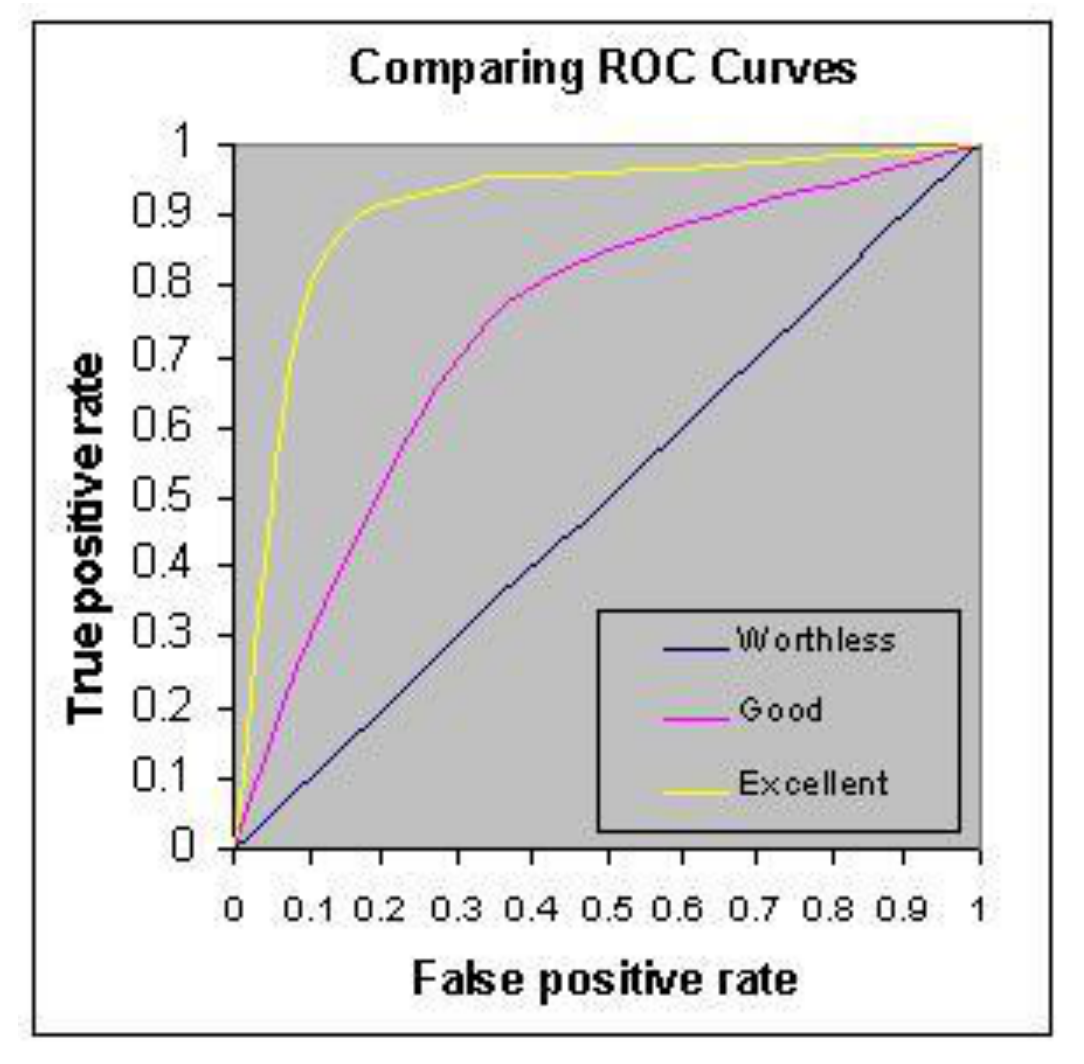
\includegraphics[width=\textwidth,height=4.8cm,keepaspectratio]{images/slide60_roc_comparison_plot.png}
      \end{center}
    \end{column}
  \end{columns}
\end{frame}
